\documentclass{article}
\usepackage[english,russian]{babel}
\usepackage{textcomp}
\usepackage{geometry}
  \geometry{left=2cm}
  \geometry{right=1.5cm}
  \geometry{top=1.5cm}
  \geometry{bottom=2cm}
\usepackage{tikz}
\usepackage{multicol}
\usepackage{hyperref}
\usepackage{listings}
\pagenumbering{gobble}

\lstdefinestyle{csMiptCppStyle}{
  language=C++,
  basicstyle=\linespread{1.1}\ttfamily,
  columns=fixed,
  fontadjust=true,
  basewidth=0.5em,
  keywordstyle=\color{blue}\bfseries,
  commentstyle=\color{gray},
  texcl=true,
  stringstyle=\ttfamily\color{orange!50!black},
  showstringspaces=false,
  numbersep=5pt,
  numberstyle=\tiny\color{black},
  numberfirstline=true,
  stepnumber=1,      
  numbersep=10pt,
  backgroundcolor=\color{white},
  showstringspaces=false,
  captionpos=b,
  breaklines=true
  breakatwhitespace=true,
  xleftmargin=.2in,
  extendedchars=\true,
  keepspaces = true,
  tabsize=4,
  upquote=true,
}


\lstdefinestyle{csMiptCppLinesStyle}{
  style=csMiptCppStyle,
  frame=lines,
}

\lstdefinestyle{csMiptCppBorderStyle}{
  style=csMiptCppStyle,
  framexleftmargin=5mm, 
  frame=shadowbox, 
  rulesepcolor=\color{gray}
}


\lstdefinestyle{csMiptBash}{
breaklines=true,
frame=tb,
language=bash,
breakatwhitespace=true,
alsoletter={*()"'0123456789.},
alsoother={\{\=\}},
basicstyle={\ttfamily},
keywordstyle={\bfseries},
literate={{=}{{{=}}}1},
prebreak={\textbackslash},
sensitive=true,
stepnumber=1,
tabsize=4,
morekeywords={echo, function},
otherkeywords={-, \{, \}},
literate={\$\{}{{{{\bfseries{}\$\{}}}}2,
upquote=true,
frame=none
}


\lstset{style=csMiptCppLinesStyle}
\lstset{literate={~}{{\raisebox{0.5ex}{\texttildelow}}}{1}}


\renewcommand{\thesection}{\arabic{section}}
\makeatletter
\def\@seccntformat#1{\@ifundefined{#1@cntformat}%
   {\csname the#1\endcsname\quad}%    default
   {\csname #1@cntformat\endcsname}}% enable individual control
\newcommand\section@cntformat{Часть \thesection:\space}
\makeatother



\begin{document}
\title{Семинар \#0: Основы командной строки и git \vspace{-5ex}}\date{}\maketitle

\section*{Основные команды терминала Linux}
\texttt{
\begin{tabular}{ l | l }
 pwd                     			& напечатать имя текущей директории \\ 
 ls                      			& напечатать все файлы и папки текущей директории \\ 
 ls -l                      		& больше информации \\ 
 ls -a                      		& показать скрытые файлы \\ 
 cd имя\_папки          			& перейти в соответствующую папку \\
                         			& например:  cd /home-local/student \\ 
 cd ..         						& перейти в папку, содержащую данную \\ \hline
 mkdir имя\_новой\_папки 			& создать новую папку \\
 touch имя\_нового\_файла 			& создать новый пустой файл \\
 cp имя\_файла новое\_расположение 	& копировать файл \\
 mv имя\_файла новое\_расположение 	& переместить файл \\
 mv имя\_файла новое\_имя\_файла 	& переименовать файл \\
 rm имя\_файла  					& удалить файл \\
 rm -r имя\_папки  					& удалить папку \\
\end{tabular}
}

\subsection*{Сокращение для имён папок}
\texttt{
\begin{tabular}{ l | l }
 .                     			& текущая директория \\ 
 ..                     		& родительская директория \\ 
 $\sim$                     	& домашняя директория (на linux это \texttt{/home/<имя>}, на windows \texttt{С:\textbackslash Users\textbackslash <имя>})\\ 
\end{tabular}
}


\subsection*{Горячие клавиши}
\texttt{
\begin{tabular}{ l | l }
 Tab           & автозаполнение \\ 
 2 раза Tab    & показать возможные варианты \\ 
 стрелка вверх & перейти к предыдущей команде \\ 
 Ctrl-C        & выход из программы, например той, которая зависла в бесконечном цикле \\ 
 Ctrl-D        & конец ввода \\ 
 Ctrl-R        & поиск по всем предыдущим командам \\ 
\end{tabular}
}



\subsection*{Компиляция программы на языке C}
\texttt{
\begin{tabular}{ l | l }
 gcc имя\_файла\_исходного\_кода  	& скомпилировать программу и создать исполняемый файл \texttt{a.out}\\
 ./a.out                         	& запустить файл a.out в текущей директории \
\end{tabular}
}

\begin{center}
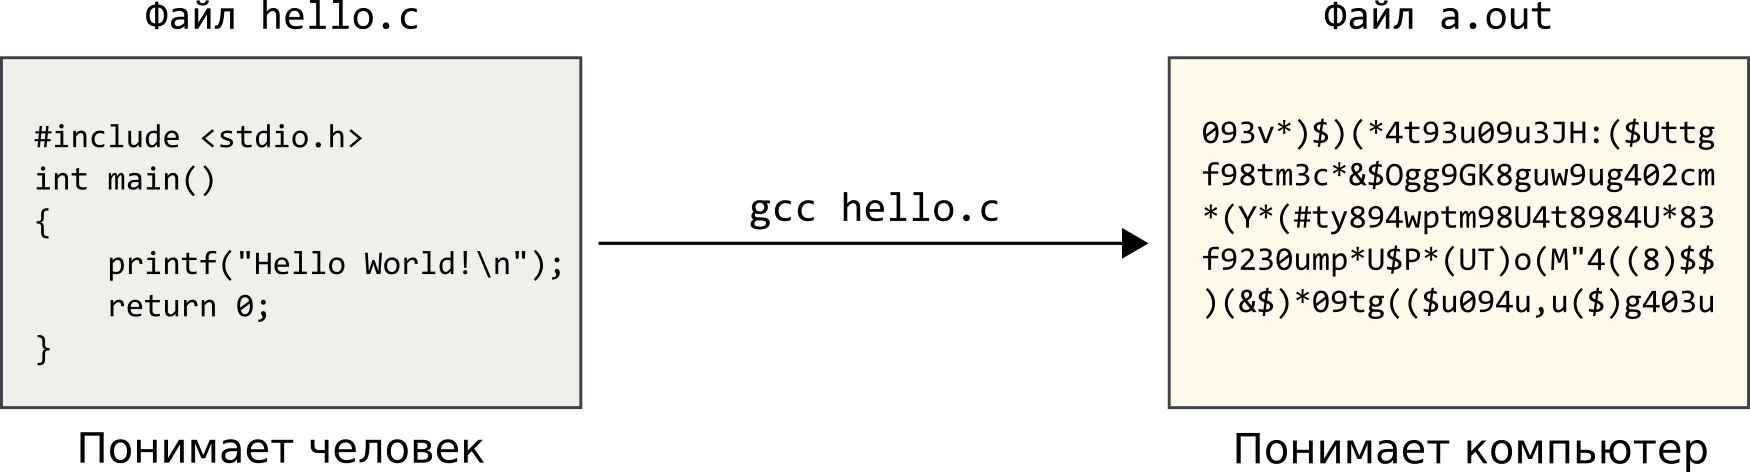
\includegraphics[scale=1]{../images/gcc_simple.png}
\end{center}


\subsection*{Запуск скрипта Python}
\texttt{
\begin{tabular}{ l | l }
 python имя\_скрипта  	& запустить скрипт\\
\end{tabular}
}


\subsection*{Работа с текстом}
\texttt{
\begin{tabular}{ l | l }
 nano имя\_файла  	& открыть файл в редакторе nano, если файла не существует, то будет создан новый\\
   				  	& Ctrl-O - для сохранения изменений\\
   				  	& Ctrl-X - для выхода\\
\end{tabular}
}


\subsection*{Работа с ssh}
\texttt{
\begin{tabular}{ l | l }
 ssh-keygen 				& создаёт публичный и приватный ssh-ключи в папке $\sim$/.ssh\\
 							& во время запуска попросит ввести passphrase, можно ничего не вводить\\
 							& публичный ключ будет иметь расширение .pub, этот ключ можно передавать другим\\
 							& приватный ключ будет без расширения, его нельзя показывать никому\\
 							& после создания, вам нужно скопировать публичный ключ в настройки gitlab или github,\\
 							& тогда вы сможете делать команды git push и git pull\\
\end{tabular}
}



\section*{Основы git}

\subsection*{Создание репозитория}
\texttt{
\begin{tabular}{ l | l }
 git init                     			& создать новый пустой репозиторий в данной папке \\ 
 git clone путь\_до\_репозитория          & клонировать репозиторий \\ 
\end{tabular}
}

\subsection*{Настройки}
\texttt{
\begin{tabular}{ l | l }
 git config --global user.name "ваше имя" & настройка имени \\ 
 git config --global user.email "ваш адрес почты" & настройка почты \\ 
 git config --global core.editor "nano" & установка текстового редактора nano редактором\\
                                        & по умолчанию для git \\ 
\end{tabular}
}

\subsection*{Добавление изменений в локальный репозиторий}
\texttt{
\begin{tabular}{ l | l }
 git add имена\_файлов					& добавить файлы в индекс\\
 git add --all							& добавить все изменения (новые, изменённые, удалённые файлы) в индекс\\ \hline
 git commit							    & добавить все изменения, добавленные в индекс с момента прошлого коммита,\\
 										& в локальный репозиторий, после этого откроется текстовый редактор куда\\
 										& нужно будет написать сообщение о коммите и закрыть его.\\
 git commit -m "сообщение"    & то же, но без открытия редактора\\
\end{tabular}
}


\subsection*{Просмотр информации о добавленных изменениях}
\texttt{
\begin{tabular}{ l | l }
 git status 							& показывает произведённые изменения в рабочей папке и в индексе\\
 										& изменения сделанные в папке, но не добавленные в индекс пишутся красным\\
 										& изменения добавленные в индекс, но не в лок. репозиторий пишутся зелёным\\ \hline
 git log								& показывают информацию о произведённых коммитах\\
 git log --oneline						& сокращённая запись\\
 git log --graph --oneline --all		& рисует весь граф коммитов\\
\end{tabular}
}


\subsection*{Добавление изменений из локального репозитория в удалённый}

\texttt{
\begin{tabular}{ l | l }
 git remote -v							& просмотр списка удалённых репозиториев \\
 git remote add  						& добавить новый удалённый сервер\\
 \quad \quad имя\_уд.репозитория адрес	& 1) имя удалённого сервера можно задать любым, но обычно\\
 										& используется имя origin.\\
 										& 2) если вы работаете на gitlab или github то адрес можно найти там\\
 										& кнопка Code на этих сайтах, лучше использовать протокол SSH.\\ \hline
 git push имя\_уд.\_сервера		& отправка изменений из локального репозитория в удалённый (текущая ветка)\\
 git pull имя\_уд.\_сервера			& получение изменений из удалённого репозитория (все ветки) + слияние (текущая ветка)\\
\end{tabular}
}


\end{document}
